% Carátula para el manual del usuario
\documentclass[a4paper,12pt]{article}
\usepackage[spanish]{babel}
\usepackage[utf8]{inputenc}
\usepackage{graphicx}
\usepackage{geometry}
\usepackage{xcolor} % Added package for \textcolor command
\usepackage[colorlinks=true, linkcolor=black, urlcolor=black]{hyperref}
\geometry{top=2.5cm, bottom=2.5cm, left=2.5cm, right=2.5cm}

\begin{document}

% Logo arriba a la derecha
\begin{flushright}
    \includegraphics[width=4cm]{apipmusiclogo.png} % Logo del proyecto
\end{flushright}

\vspace*{2cm}

\begin{center}
    {\LARGE\bfseries Manual del Usuario} \\[1.5cm]
    \textbf{Integrantes:} \\[0.3cm]
    Santiago Ibarra \\[0.2cm]
    Agustin Colman \\[0.2cm]
    Carlos Insaurralde \\[0.2cm]
    Gabriel Beneitez \\[1.2cm]
    Curso: 7°2 \\
    \vspace{0.5cm}
    \textbf{Materia:} Proyecto de Desarrollo de Software para Plataformas Móviles
\end{center}

\vfill

\begin{center}
    \textit{Escuela de Educación Secundaria Técnica N°1} \\
    \textit{Año 2025}
\end{center}

\thispagestyle{empty}
\newpage

% Índice de contenidos con enlaces
\tableofcontents
\newpage

% ===============================
% 1. Introducción
% ===============================
\section{Introducción}
Bienvenido al manual de usuario del ``Reproductor Inteligente", una aplicación diseñada para seleccionar música que se adapte a tu ritmo cardíaco durante el ejercicio. Esta aplicación te permite simular tus pulsaciones por minuto (PPM) y recibir recomendaciones de canciones con ritmos similares, optimizando así tu experiencia de entrenamiento.

% Aquí iría una imagen de la pantalla principal de la aplicación
\begin{figure}[h]
    \centering
    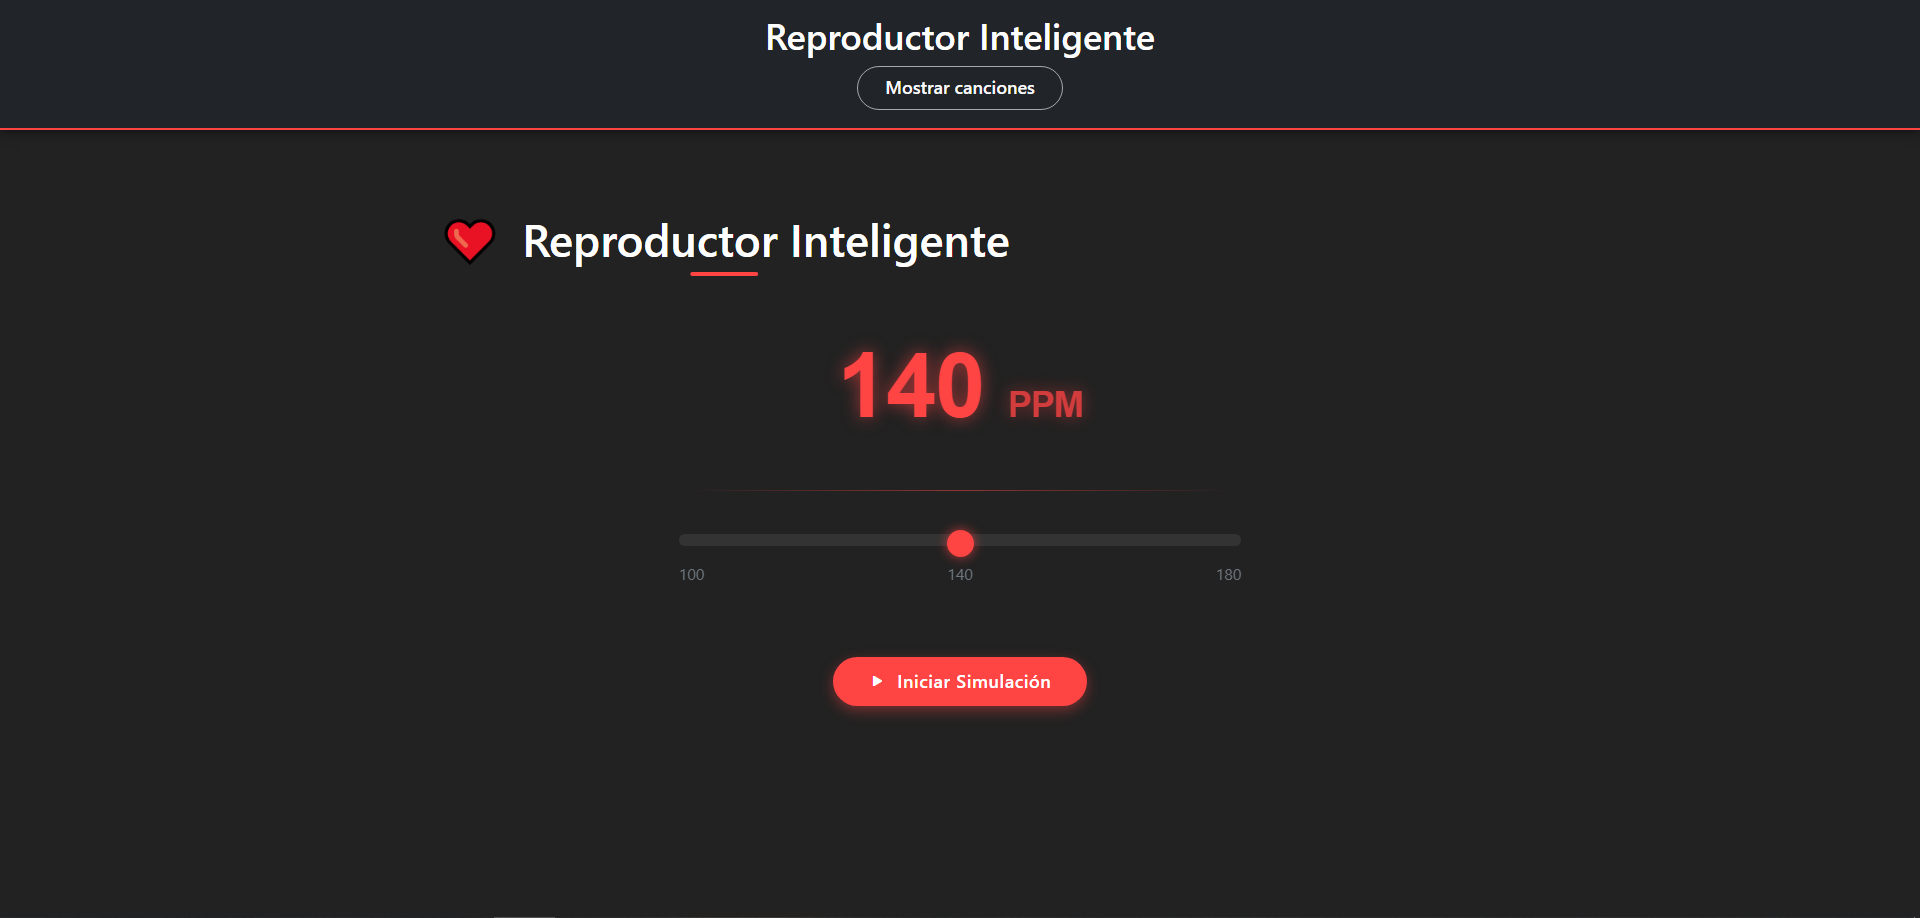
\includegraphics[width=0.8\textwidth]{imagenes/pantalla_principal.png}
    \caption{Pantalla principal del Reproductor Inteligente}
\end{figure}

% ===============================
% 2. Requisitos del Sistema
% ===============================
\section{Requisitos del Sistema}
Para utilizar el Reproductor Inteligente, necesitarás:
\begin{itemize}
    \item Un navegador web actualizado (Chrome, Firefox, Edge o Safari)
    \item Conexión a Internet para cargar las canciones
    \item Dispositivo con capacidad de reproducción de audio
\end{itemize}

% ===============================
% 3. Acceso a la Aplicación
% ===============================
\section{Acceso a la Aplicación}
Para acceder al Reproductor Inteligente:
\begin{enumerate}
    \item Abre tu navegador web
    \item Ingresa la dirección URL proporcionada por tu instructor
    \item La aplicación se cargará automáticamente mostrando la pantalla principal
\end{enumerate}

% Aquí iría una imagen del navegador con la URL
 \begin{figure}[h]
     \centering
     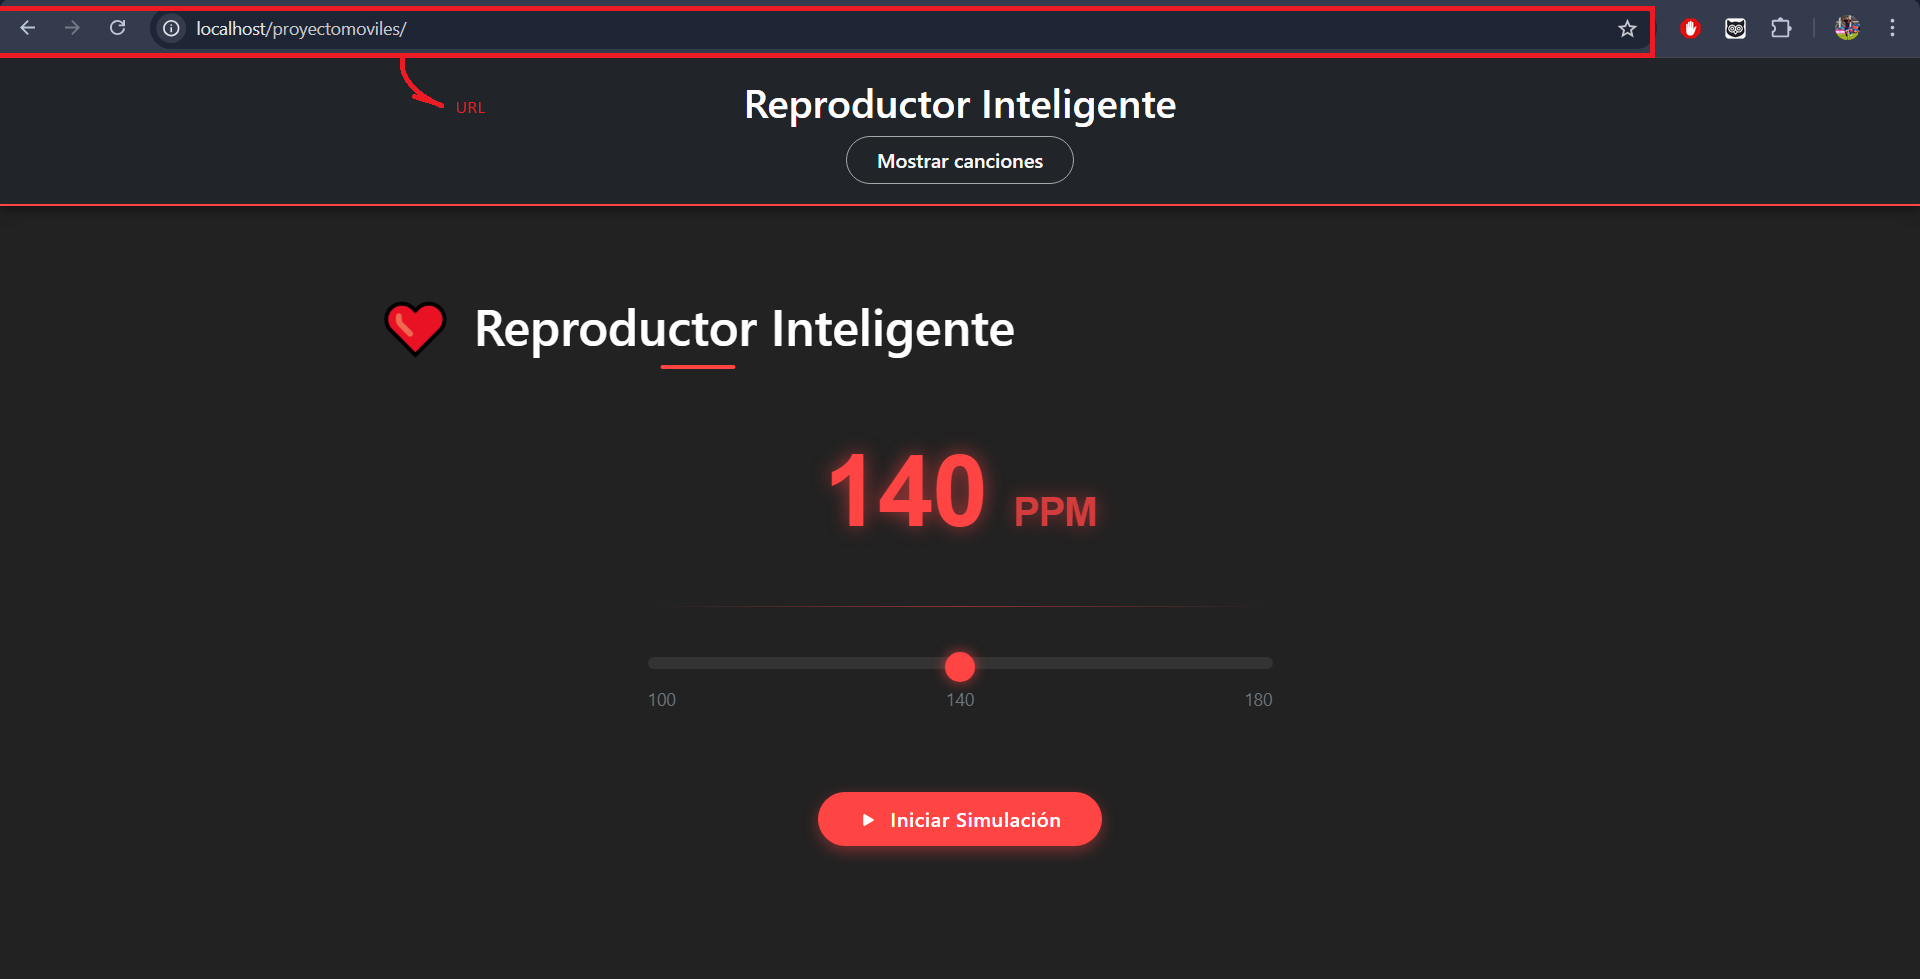
\includegraphics[width=0.8\textwidth]{imagenes/acceso_navegador.png}
     \caption{Acceso a la aplicación desde el navegador}
 \end{figure}

% ===============================
% 4. Interfaz de Usuario
% ===============================
\section{Interfaz de Usuario}
La interfaz del Reproductor Inteligente está diseñada para ser intuitiva y fácil de usar. A continuación, se describen los principales elementos:

\subsection{Barra de Navegación}
En la parte superior de la pantalla encontrarás:
\begin{itemize}
    \item El título ``Reproductor Inteligente"
    \item Un botón ``Mostrar canciones" que te llevará al listado completo de canciones disponibles
\end{itemize}

% Aquí iría una imagen de la barra de navegación
 \begin{figure}[h]
     \centering
     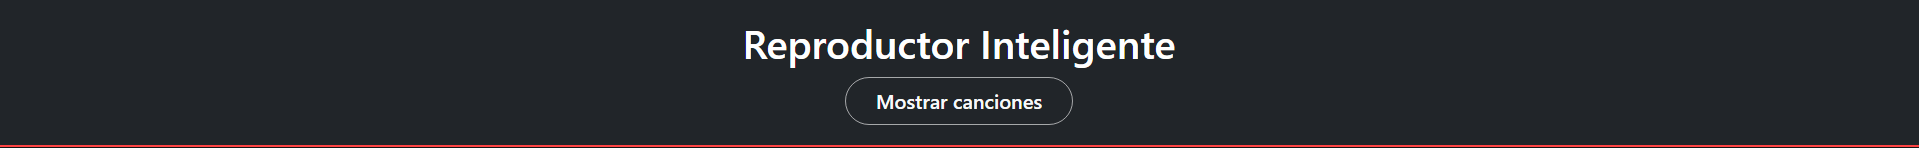
\includegraphics[width=0.8\textwidth]{imagenes/barra_navegacion.png}
     \caption{Barra de navegación}
 \end{figure}

\subsection{Control de PPM}
En la sección central de la pantalla encontrarás:
\begin{itemize}
    \item Un indicador numérico que muestra tu PPM actual
    \item Un control deslizante para ajustar manualmente tu PPM
    \item Un botón ``Iniciar Simulación" para comenzar la simulación automática de PPM
\end{itemize}

% Aquí iría una imagen del control de PPM
 \begin{figure}[h]
     \centering
     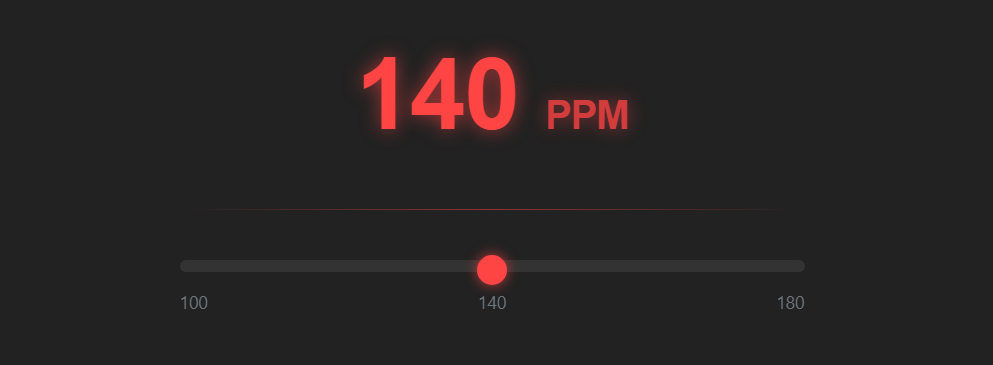
\includegraphics[width=0.6\textwidth]{imagenes/control_ppm.png}
     \caption{Control de PPM}
 \end{figure}

%\subsection{Recomendaciones de Canciones}
%Debajo del control de PPM, verás:
%\begin{itemize}
%    \item Tarjetas con canciones recomendadas según tu PPM actual
%    \item Cada tarjeta muestra el nombre de la canción, artista, año y PPM
%    \item Un botón ``Reproducir" para escuchar la canción
%\end{itemize}

% Aquí iría una imagen de las recomendaciones
% \begin{figure}[h]
%     \centering
%     \includegraphics[width=0.8\textwidth]{imagenes/recomendaciones.png}
%     \caption{Recomendaciones de canciones}
% \end{figure}

\subsection{Reproductor Actual}
Cuando reproduces una canción, aparece una sección que muestra:
\begin{itemize}
    \item Información detallada de la canción en reproducción
    \item Una barra de progreso que indica el avance de la canción
    \item El tiempo actual y duración total
\end{itemize}

% Aquí iría una imagen del reproductor
 \begin{figure}[h]
     \centering
     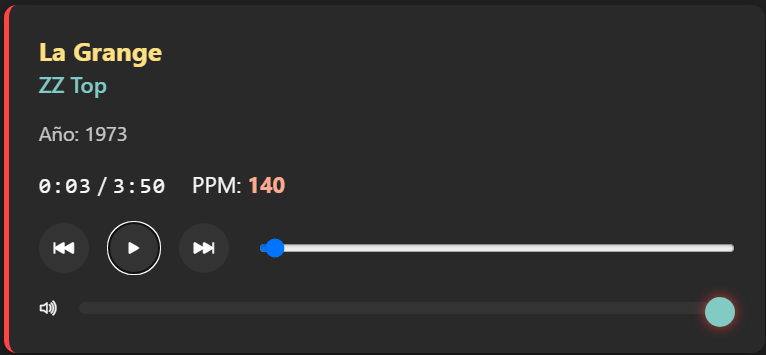
\includegraphics[width=0.7\textwidth]{imagenes/reproductor.png}
     \caption{Reproductor de la canción actual}
 \end{figure}

\subsection{Historial de Reproducción}
En la esquina superior derecha encontrarás:
\begin{itemize}
    \item Un panel que muestra las últimas canciones reproducidas
    \item Se actualiza automáticamente al reproducir nuevas canciones
\end{itemize}

% Aquí iría una imagen del historial
 \begin{figure}[h]
     \centering
     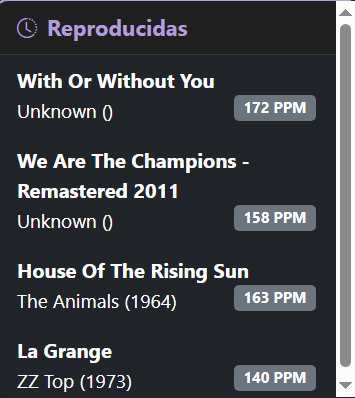
\includegraphics[width=0.4\textwidth]{imagenes/historial.png}
     \caption{Historial de reproducción}
 \end{figure}

% ===============================
% 5. Uso de la Aplicación
% ===============================
\section{Uso de la Aplicación}

\subsection{Ajuste Manual de PPM}
Para ajustar manualmente tu PPM:
\begin{enumerate}
    \item Desliza el control deslizante hacia la izquierda para disminuir el PPM
    \item Desliza el control deslizante hacia la derecha para aumentar el PPM
    \item Observa cómo las recomendaciones de canciones se actualizan automáticamente
\end{enumerate}

% Aquí iría una imagen del ajuste manual
 \begin{figure}[h]
     \centering
     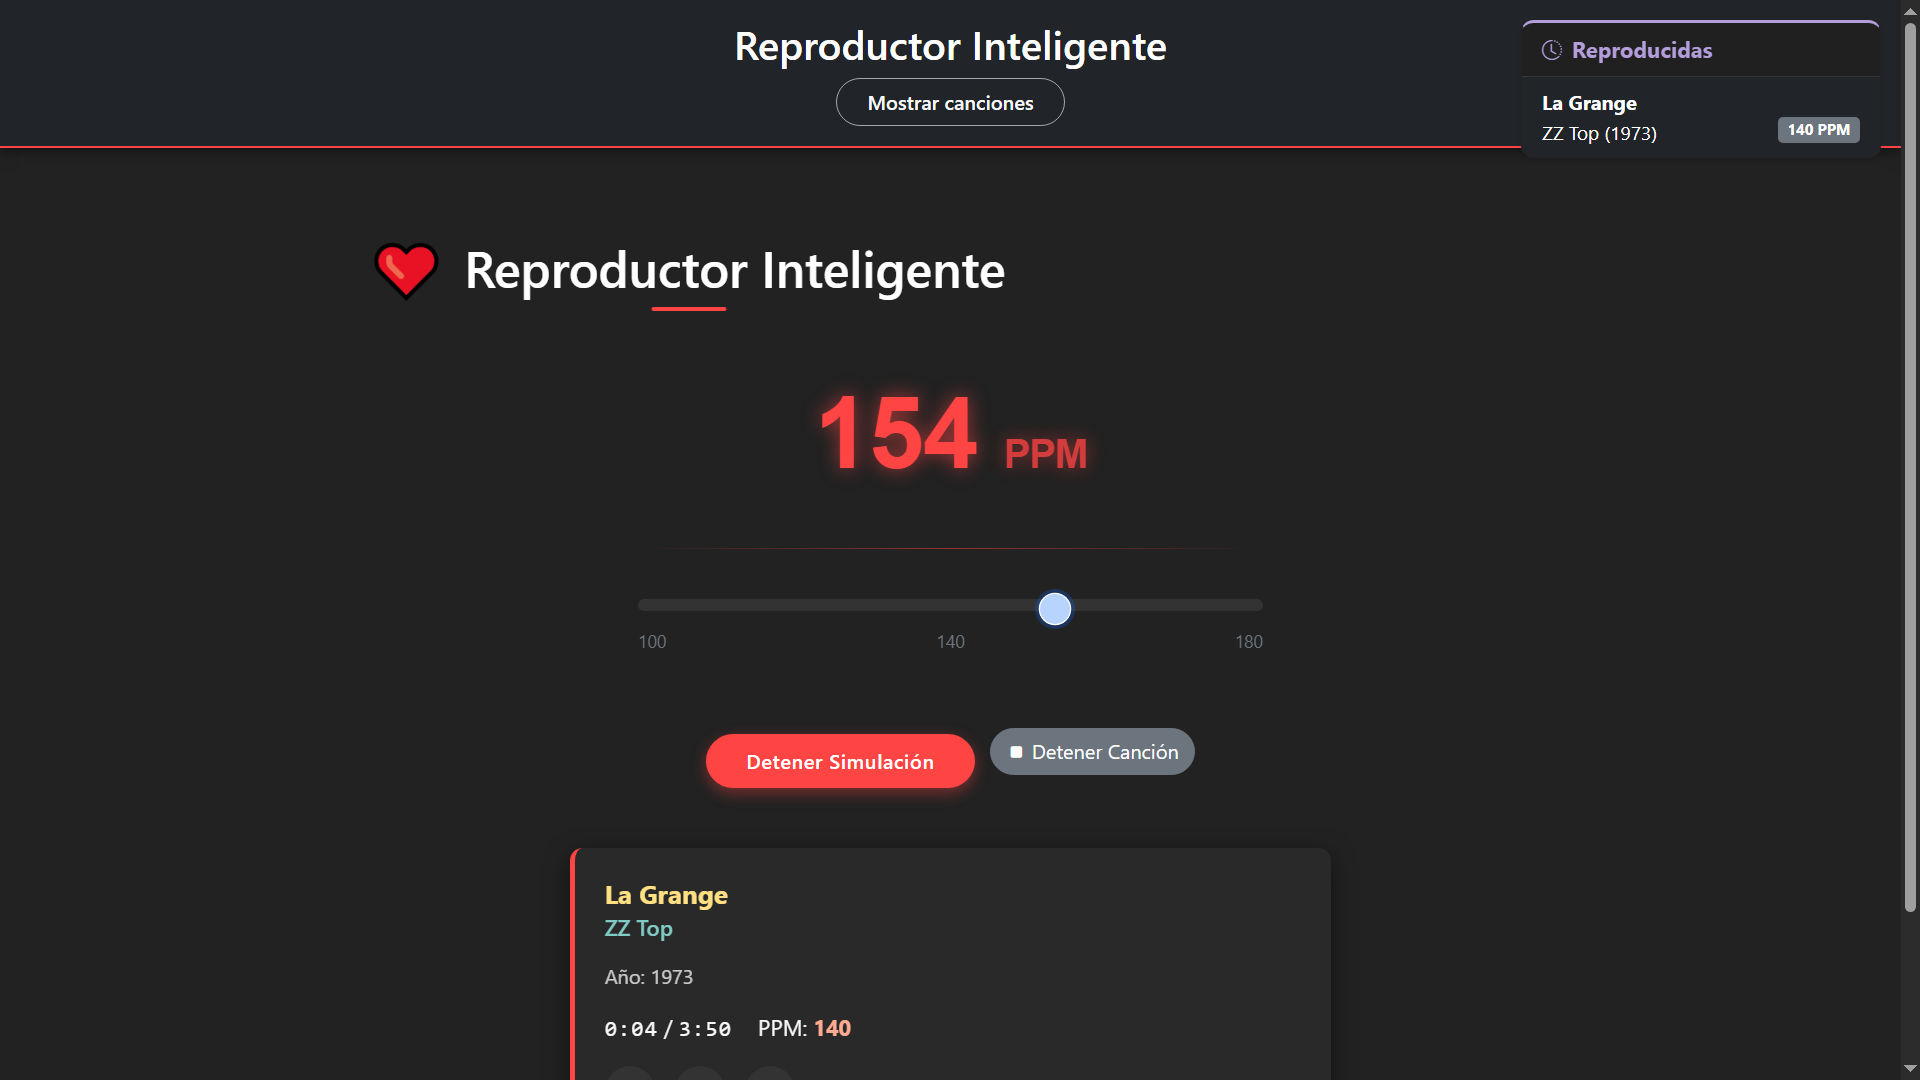
\includegraphics[width=0.6\textwidth]{imagenes/ajuste_manual.png}
     \caption{Ajuste manual del PPM}
 \end{figure}

\subsection{Simulación de PPM}
Para simular automáticamente cambios en tu PPM:
\begin{enumerate}
    \item Haz clic en el botón ``Iniciar Simulación"
    \item Observa cómo el valor de PPM cambia automáticamente, simulando variaciones naturales durante el ejercicio
    \item Las recomendaciones de canciones se actualizarán según el PPM simulado
    \item Para detener la simulación, haz clic en el botón ``Detener Simulación"
\end{enumerate}

% Aquí iría una imagen de la simulación
% \begin{figure}[h]
%     \centering
%     \includegraphics[width=0.6\textwidth]{imagenes/simulacion.png}
%     \caption{Simulación de PPM en funcionamiento}
% \end{figure}

%\subsection{Reproducción Manual de Canciones}
%Para reproducir una canción manualmente:
%\begin{enumerate}
%    \item Busca una canción que te interese en las recomendaciones
%    \item Haz clic en el botón ``Reproducir" de esa canción
%    \item La canción comenzará a reproducirse y aparecerá en el reproductor actual
%    \item Para pausar la reproducción, haz clic nuevamente en el botón (ahora muestra ``Pausar")
%\end{enumerate}

% Aquí iría una imagen de la reproducción manual
% \begin{figure}[h]
%     \centering
%     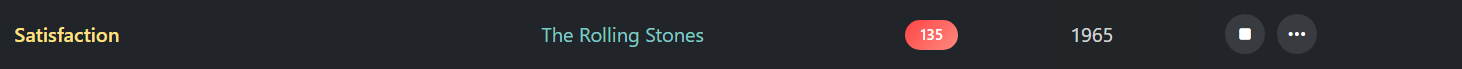
\includegraphics[width=0.7\textwidth]{imagenes/reproduccion_manual.png}
%     \caption{Reproducción manual de una canción}
% \end{figure}

\subsection{Reproducción Automática}
Durante la simulación de PPM, la aplicación puede reproducir canciones automáticamente:
\begin{enumerate}
    \item Inicia la simulación de PPM como se explicó anteriormente
    \item La aplicación seleccionará y reproducirá automáticamente canciones que coincidan con tu PPM actual
    \item Cuando termine una canción, se seleccionará automáticamente otra con un PPM similar
    \item Para detener la reproducción automática, detén la simulación
\end{enumerate}

% Aquí iría una imagen de la reproducción automática
 \begin{figure}[h]
     \centering
     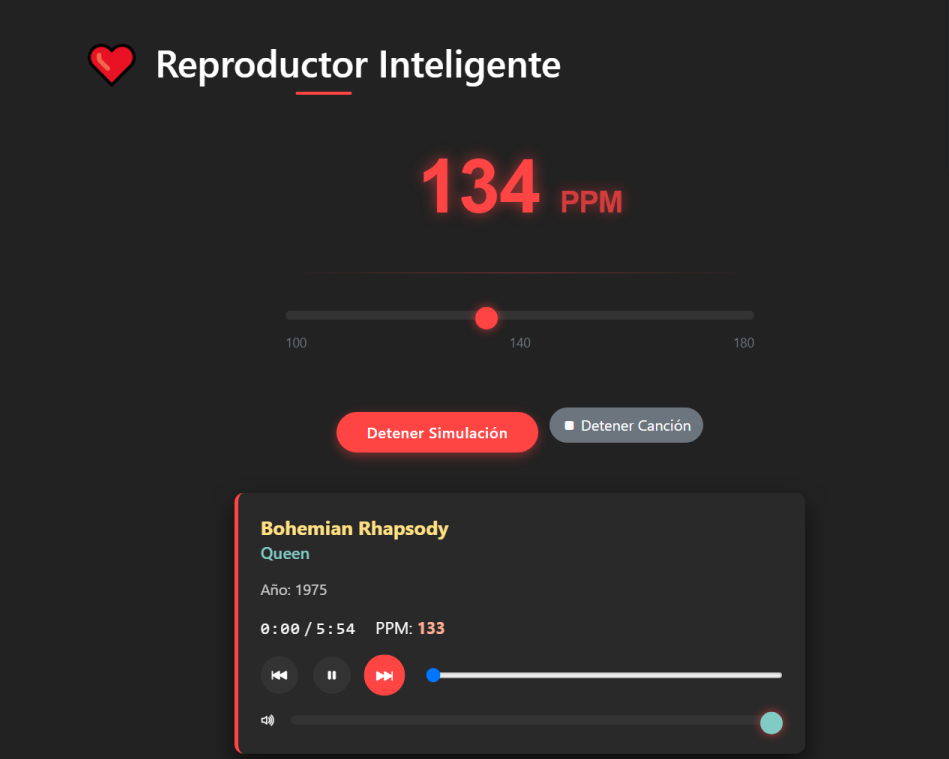
\includegraphics[width=0.7\textwidth]{imagenes/reproduccion_automatica.png}
     \caption{Reproducción automática durante la simulación}
 \end{figure}

\subsection{Control de Volumen}
Para ajustar el volumen de reproducción:
\begin{enumerate}
    \item Localiza el control deslizante de volumen en la parte inferior de la pantalla
    \item Desliza hacia la izquierda para disminuir el volumen
    \item Desliza hacia la derecha para aumentar el volumen
\end{enumerate}

% Aquí iría una imagen del control de volumen
 \begin{figure}[h]
     \centering
     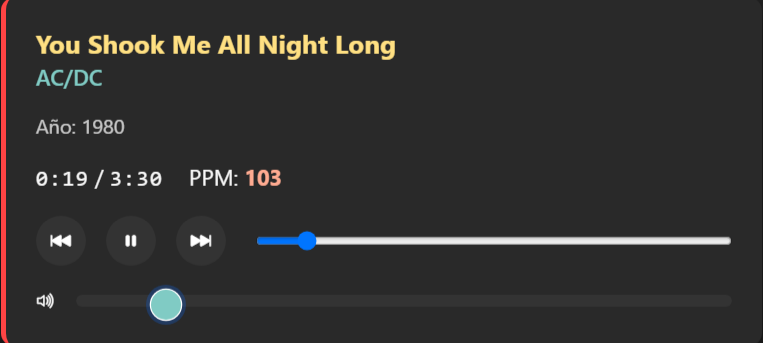
\includegraphics[width=0.5\textwidth]{imagenes/control_volumen.png}
     \caption{Control de volumen}
 \end{figure}

\subsection{Visualización del Listado Completo}
Para ver todas las canciones disponibles:
\begin{enumerate}
    \item Haz clic en el botón ``Mostrar canciones" en la barra de navegación
    \item Se abrirá una nueva página con una tabla que muestra todas las canciones
    \item Puedes reproducir cualquier canción directamente desde esta lista
    \item Para volver al reproductor principal, utiliza el botón de navegación del navegador o haz clic en el título
\end{enumerate}

\subsubsection{Búsqueda y Filtros}
El listado de canciones ofrece varias opciones para encontrar rápidamente la música que deseas:

\begin{enumerate}
    \item \textbf{Búsqueda por texto:} Escribe en el campo de búsqueda para filtrar canciones por título o artista
    \item \textbf{Filtro por PPM:} Selecciona un rango de PPM del menú desplegable:
    \begin{itemize}
        \item Bajo (100-120 PPM)
        \item Medio (121-150 PPM)
        \item Alto (151-180 PPM)
    \end{itemize}
    \item \textbf{Ordenamiento:} Ordena las canciones por diferentes criterios:
    \begin{itemize}
        \item Título (A-Z o Z-A)
        \item Artista (A-Z o Z-A)
        \item PPM (Menor a Mayor o Mayor a Menor)
        \item Año (Antiguo a Reciente o Reciente a Antiguo)
    \end{itemize}
    \item \textbf{Botón Resetear:} Elimina todos los filtros aplicados y muestra nuevamente todas las canciones
\end{enumerate}
\begin{figure}[h]
    \centering
    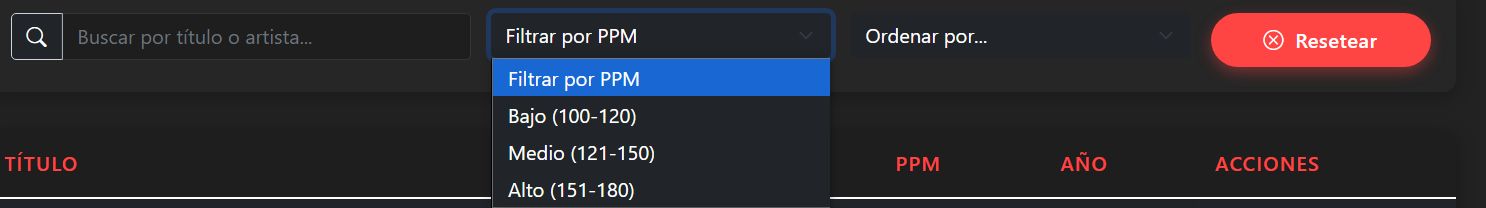
\includegraphics[width=0.7\textwidth]{imagenes/barra_canciones.png}
    \caption{Barra de filtros}
\end{figure}


\subsubsection{Reproducción de Canciones}
Para reproducir una canción desde el listado:

\begin{enumerate}
    \item Localiza la canción deseada en la tabla
    \item Haz clic en el botón de reproducción (ícono de play) junto a la canción
    \item Para detener la reproducción, haz clic en el botón de detener (ícono de stop) que aparece
\end{enumerate}

\begin{figure}[h]
    \centering
    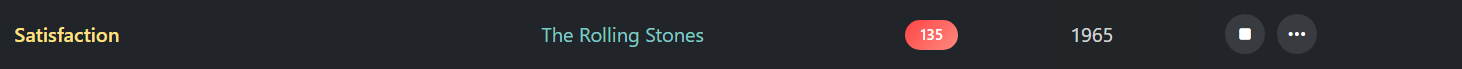
\includegraphics[width=0.7\textwidth]{imagenes/reproduccion_manual.png}
    \caption{Reproducción manual de una canción}
\end{figure}

\subsubsection{Opciones Adicionales}
Cada canción cuenta con un menú de opciones adicionales:

\begin{enumerate}
    \item Haz clic en el botón de tres puntos junto a la canción
    \item Se abrirá un menú con opciones como:
    \begin{itemize}
        \item Añadir a playlist
        \item Descargar
        \item Compartir
    \end{itemize}
\end{enumerate}

\subsubsection{Navegación entre Páginas}
Cuando hay muchas canciones, el listado se divide en páginas para facilitar la navegación:

\begin{enumerate}
    \item En la parte inferior de la tabla encontrarás botones de paginación
    \item Haz clic en los números para ir a una página específica
    \item Utiliza los botones ``Anterior" y ``Siguiente" para navegar secuencialmente
    \item La página actual se muestra resaltada
\end{enumerate}

% ===============================
% 6. Preguntas Frecuentes
% ===============================
\section{Preguntas Frecuentes}

\subsection{¿Cómo funciona la recomendación de canciones?}
El sistema busca canciones cuyo PPM (pulsaciones por minuto) sea similar al PPM que estás simulando o has seleccionado manualmente. Se consideran canciones con un PPM de ±5 latidos respecto a tu PPM actual.

\subsection{¿Puedo usar la aplicación sin conexión a Internet?}
No, la aplicación necesita conexión a Internet para cargar las canciones desde el servidor.

\subsection{¿Por qué no escucho ningún sonido?}
Verifica lo siguiente:
\begin{itemize}
    \item El volumen de tu dispositivo está activado
    \item El control deslizante de volumen en la aplicación no está al mínimo
    \item Tu navegador tiene permisos para reproducir audio
    \item Los archivos de audio están disponibles en el servidor
\end{itemize}

\subsection{¿Cómo puedo añadir mis propias canciones?}
La adición de nuevas canciones debe ser realizada por el administrador del sistema. Contacta con el administrador si deseas sugerir nuevas canciones.

% ===============================
% 7. Solución de Problemas
% ===============================
\section{Solución de Problemas}

\subsection{La aplicación no carga}
\begin{itemize}
    \item Verifica tu conexión a Internet
    \item Intenta actualizar la página (F5)
    \item Prueba con otro navegador
    \item Limpia la caché del navegador
\end{itemize}

\subsection{No se muestran recomendaciones}
\begin{itemize}
    \item Puede que no haya canciones en la base de datos con un PPM similar al actual
    \item Verifica que la conexión al servidor esté funcionando correctamente
    \item Intenta ajustar el PPM a un valor diferente
\end{itemize}

\subsection{La simulación no funciona}
\begin{itemize}
    \item Asegúrate de haber hecho clic en ``Iniciar Simulación"
    \item Verifica que el navegador no esté en modo de ahorro de energía o con pestañas inactivas
    \item Actualiza la página e intenta nuevamente
\end{itemize}

% ===============================
% 8. Contacto y Soporte
% ===============================
\section{Contacto y Soporte}
Si encuentras algún problema o tienes sugerencias para mejorar la aplicación, puedes contactar con el equipo de desarrollo:

\begin{itemize}
    \item \textbf{Desarrolladores:} Santiago Ibarra, Agustin Colman, Carlos Insaurralde, Gabriel Beneitez
    \item \textbf{Curso:} 7°2 -- Año 2025
    \item \textbf{Institución:} Escuela de Educación Secundaria Técnica N°1
\end{itemize}

\end{document}
